
\documentclass[a4paper,12pt]{scrartcl}
\usepackage[utf8]{inputenc}
\usepackage[ngerman]{babel}
\usepackage[T1]{fontenc}
\usepackage{amsmath}
\usepackage{graphicx}
\usepackage{amstext}
\usepackage{caption, booktabs}
\usepackage{amssymb}
\usepackage{a4wide}
\usepackage{verbatim}
\usepackage{url}
\usepackage{setspace}
\usepackage[decimalsymbol=comma]{siunitx}
\sisetup{separate-uncertainty}
\usepackage{subfigure}
\usepackage{subfig}
\usepackage{caption}
\usepackage{placeins}
\usepackage{floatrow}
\newcommand{\q}[2]{#1_{\mathrm{#2}}}

\floatsetup[table]{capposition=top}

\begin{document}
\begin{titlepage}


\title{Geoelektrik}



\vfill
\maketitle
\end{titlepage}
\newpage
\tableofcontents
\newpage
\section{Einführung}
Mit geoelektrischen Messungen werden Materialeigenschaften wie die Ionenkonzentration, Grad der Wassersättigung und der Permeabilität untersucht. 
Das bedeutet dass mit Hilfe dieses Verfahrens z.B der Grundwasserspiegel bestimmt werden kann. \\
Während der Geländeübung wird mit dem geoelektrischen Gleichstromverfahren eine Kartierung der Leitfähigkeit des Untergrunds erstellt.

\section{Theoretische Grundlagen}
Während der Geländeübung werden die Messungen mit dem Gleichstromverfahren durchgeführt. Dabei wird an zwei Elektroden Gleichstrom angelegt,
über zwei Sonden an der Oberfläche wird die Spannung gemessen. Mit diesem Verfahren wird also die Materialeigenschaft elektrischen Strom zu leiten untersucht. \\
Hierbei unterscheidet man zwischen elektrischer Leitfähigkeit, wenn Elektronen bewegt werden, und ionischer Leitfähigkeit, dem Transport von Ionen. 
Aufgrund der elektrischen Leitfähigkeit können z.B Metallrohre im Boden lokalisiert werden. Ionische Leitfähigkeit tritt in Gesteinen und Lockersedimenten auf,die einen entsprechenden Wassergehalt haben. \\
\\
Als Materialeigenschaft wird der spezifischen Widerstands $$[\rho] = \SI{1}{\Omega m}$$ bestimmt, er ist der Kehrwert der Leitfähigkeit $\sigma$.

\subsection{Wenner-Anordnung und Geometriefaktor}
In Abbildung \ref{abb:Wenner} ist der schematische Aufbau der Wenner-Anordnung zu sehen. Bei \textbf{A} und \textbf{B} sind die Elektroden und bei \textbf{M}, \textbf{N} die Sonden zur Spannungsmessung.

%%%%%%%%%%%%%%%%%%%%%%%%%%%%%%%%%%%%%
\begin{figure}[h]
\centering
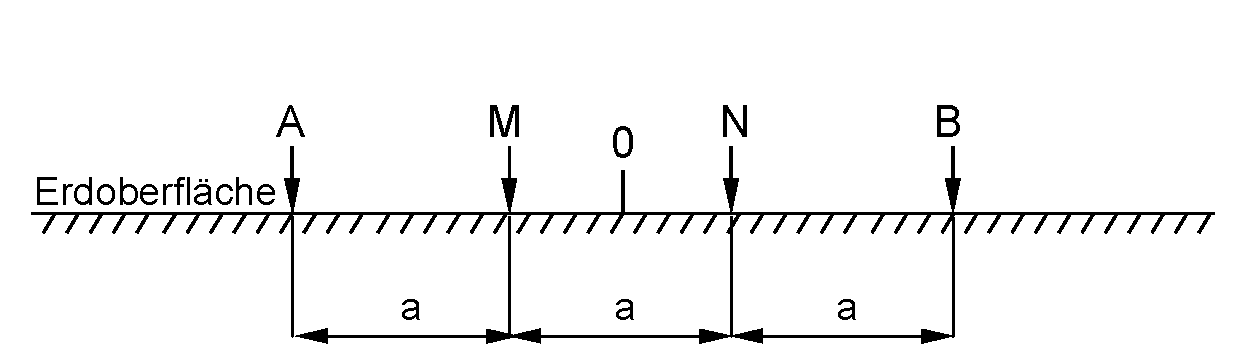
\includegraphics[width=0.6\textwidth]{Wenner.png}
\caption{Schematische Darstellung der Schlumberger-Anordnung}
\label{abb:Wenner}
\end{figure}
%%%%%%%%%%%%%%%%%%%%%%%%%%%%%%%%%%%%
Die Potentialdifferenz bei einem Angelegten Strom I ist
\begin{equation}
V = \rho \, I \, \frac{1}{2 \pi} \big(\frac{1}{r_{\mathrm{AM}}} - \frac{1}{r_{\mathrm{MB}}} + \frac{1}{r_{\mathrm{NB}}} - \frac{1}{r_{\mathrm{AN}}} \big) \, ,
\end{equation}
wobei mit $r_{\mathrm{AM}}$ usw. jeweils die Abstände zwischen den Sonden und Elektroden bezeichnet werden.
Um den spezifischen Widerstand leichter berechnen zu können wird der Geometriefaktor $F$ eingeführt,
$$F = \frac{2 \pi}{\frac{1}{r_{\mathrm{AM}}} - \frac{1}{r_{\mathrm{MB}}} + \frac{1}{r_{\mathrm{NB}}} - \frac{1}{r_{\mathrm{AN}}}}\,.$$
Damit lässt sich $\rho$ berechnen mit 
\begin{equation}
\rho = \frac{V}{I} \, F.
\end{equation} \label{eq:roh}

\textbf{Scheinbarer spezifischer Widerstand}

Ist der Untergrund nicht homogen, dann wird der Wert der Formel \ref{eq:roh} als scheinbarer spezifischer Widerstand bezeichnet. Der Geometriefaktor hängt nur von der geometrischen Anordnung ab und nicht von der 
Leitfähigkeit des Untergrunds, weshalb der scheinbare spezifische Widerstand $q_a$ nur im Falle eines homogenen Untergrunds gleich dem spezifischen Widerstands ist.\\
Im Falle der Wenner-Anordnung wird  der scheinbare spezifische Widerstand mit der Formel
$$ \rho_a = 2 \pi \frac{V}{I} a $$
berechnet.
Bei einer Messung wird versucht durch Interpretation der gemessenen scheinbaren Widerstände den spezifischen Widerstand zu finden.

\subsection{Schlumberger-Anordnung}
Die Schlumberger-Anordnung wird in der Geländeübung zur Sondierung verwendet. Es wird die Änderung des spezifischen Widerstands in den verschiedenen Schichten den Untergrunds bestimmt.

%%%%%%%%%%%%%%%%%%%%%%%%%%%%%%%%%%%%%
\begin{figure}[h]
\centering
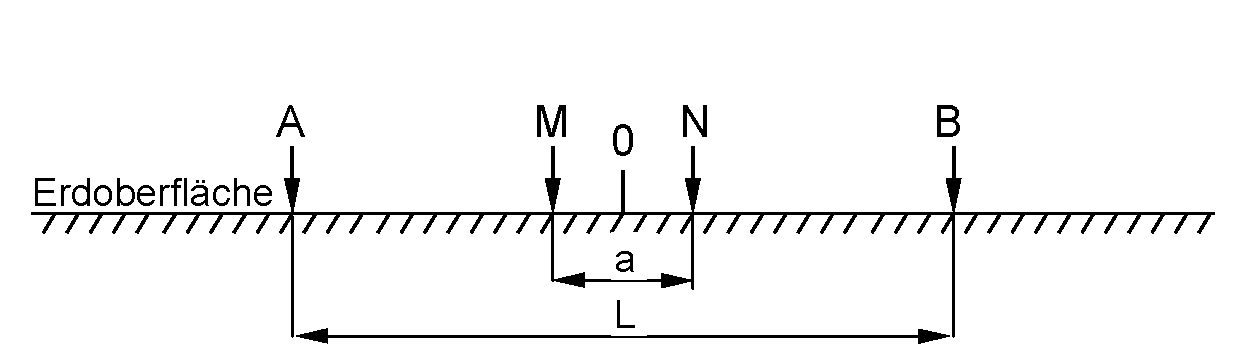
\includegraphics[width=0.6\textwidth]{Schlumberger.png}
\caption{Schematische Darstellung der Schlumberger-Anordnung}
\label{abb:Schlumberger}
\end{figure}
%%%%%%%%%%%%%%%%%%%%%%%%%%%%%%%%%%%%











%%%%%%%%%%%%%%%%%%%%%%%%%%%%%%%%
\newpage
\begin{thebibliography}{999}
\bibitem {Zitat01} \url{https://de.wikipedia.org/wiki/Geoelektrik} Datum: 06.05.18
\bibitem {Zitat02} \url{https://commons.wikimedia.org/wiki/File:Schlumberger.png} Datum 06.05.18

\end{thebibliography}
\end{document}
